% MDPI-style manuscript source for Information.
% The official MDPI class files are not bundled in this public repository.
% Before submission, place this content into the current official MDPI template
% from https://www.mdpi.com/authors/latex or add the official Definitions/ folder.

\documentclass[information,article,submit,pdftex,moreauthors]{Definitions/mdpi}
\usepackage{tabularx}
\usepackage{booktabs}

\firstpage{1}
\makeatletter
\setcounter{page}{\@firstpage}
\makeatother
\pubvolume{AUTHOR_TO_COMPLETE}
\issuenum{AUTHOR_TO_COMPLETE}
\articlenumber{AUTHOR_TO_COMPLETE}
\pubyear{2026}
\copyrightyear{2026}
\datereceived{AUTHOR_TO_COMPLETE}
\daterevised{AUTHOR_TO_COMPLETE}
\dateaccepted{AUTHOR_TO_COMPLETE}
\datepublished{AUTHOR_TO_COMPLETE}
\hreflink{https://doi.org/AUTHOR_TO_COMPLETE}

\Title{Beyond Accuracy in HR Analytics: An LLM-Assisted Multi-Agent XAI Governance Framework for Leakage-Safe Employee Performance Decision Support}

\TitleCitation{Beyond Accuracy in HR Analytics}

\newcommand{\orcidauthorA}{AUTHOR_TO_COMPLETE}
\newcommand{\orcidauthorB}{AUTHOR_TO_COMPLETE}

\Author{Muhammed Yusuf Batur $^{1,*}$\orcidA{} and Mehmet G{\"o}kt{\"u}rk $^{2}$\orcidB{}}

\AuthorNames{Muhammed Yusuf Batur and Mehmet G{\"o}kt{\"u}rk}
\AuthorCitation{Batur, M.Y.; G{\"o}kt{\"u}rk, M.}

\address{%
$^{1}$ \quad Rumeli University, AUTHOR_TO_COMPLETE; myusuf.batur@rumeli.edu.tr\\
$^{2}$ \quad Gebze Technical University, AUTHOR_TO_COMPLETE; gokturk@gtu.edu.tr}

\corres{Correspondence: myusuf.batur@rumeli.edu.tr; AUTHOR_TO_COMPLETE}

\abstract{Human-resource analytics systems are often evaluated mainly by predictive accuracy, although employee-performance decision support also requires governance evidence about leakage, explanation reliability, calibration, fairness and proxy risk, and the practical actionability of counterfactual scenarios. This study presents a leakage-aware, SHAP-based, calibration-aware, fairness/proxy-audited, actionability-constrained governance framework for employee-performance decision support. The predictive component remains a tabular XGBoost model; large language models are not used for prediction. Instead, SHAP, calibration, subgroup, proxy-risk, leakage, and counterfactual evidence are serialized into structured case-level evidence that is interpreted by a governed OpenAI explanation layer and audited by deterministic multi-agent governance components. The primary internal research model is \texttt{no\_salary\_hike\_no\_attrition\_no\_department + XGBoost}; full-feature models are retained only as leakage-warning upper-bound baselines. External evidence includes HRDataset\_v14 as an independent replication dataset with \texttt{PerformanceScore} mapped to the 2/3/4 target scale, while IBM and turnover datasets are treated only as restricted target-space or related-task robustness evidence. A final real OpenAI LLM-agent evaluation covered 80 cases, with 40 INX cases and 40 HRDataset\_v14 cases using \texttt{gpt-5.4-mini}. Automated technical checks reported no unsupported, forbidden, or missing-warning failures in that run. Nevertheless, final readiness remains \texttt{not\_ready} because high-severity proxy-risk and counterfactual-actionability blockers remain unresolved. The framework is therefore positioned as research-grade decision support, not as a deployment-ready or autonomous HR decision system.}

\keyword{HR analytics; explainable artificial intelligence; decision support systems; model governance; data leakage; SHAP; counterfactual explanations; large language models; multi-agent systems; algorithmic fairness}

\externalbibliography{yes}

\begin{document}

\section{Introduction}

Predictive analytics in human-resource settings can affect domains where errors, proxy effects, and overconfident explanations carry organizational and ethical risk. Prior work on artificial intelligence in human resources emphasizes that data-driven HR systems face small-data constraints, accountability requirements, possible employee reactions, and limitations of purely technical optimization \cite{tambe2019aihr,leichtdeobald2019hr}. For this reason, employee-performance prediction should not be assessed only by classification metrics. A responsible decision-support pipeline must also document whether the model uses outcome-proximal variables, whether probabilities are calibrated, whether subgroup performance or proxy signals create risks, whether explanations are stable, and whether counterfactual outputs describe practically actionable changes or merely technical model scenarios.

This manuscript reports a code-side evidence package for an LLM-assisted multi-agent XAI governance framework. The framework uses XGBoost as the predictive model \cite{chen2016xgboost}, SHAP as attribution evidence \cite{lundberg2017shap,lundberg2020tree}, calibration metrics \cite{guo2017calibration}, subgroup and proxy-risk audits \cite{mehrabi2021bias,barocas2023fairness}, and counterfactual actionability checks \cite{wachter2018counterfactual,karimi2022recourse}. A governed LLM layer then converts structured evidence into explanation JSON, and deterministic governance agents audit leakage, fairness/proxy risk, calibration, SHAP stability, counterfactual actionability, explanation compliance, and supervisor readiness. The LLM does not predict employee performance and is not used to invent evidence.

The contribution is not a claim that XGBoost alone is a sufficient employee-performance system. Instead, the contribution is an auditable information-systems architecture for evidence-constrained HR analytics governance. The framework demonstrates how accuracy, leakage control, calibration, XAI, counterfactual actionability, LLM explanation faithfulness, guardrail behavior, and final readiness can be tracked together. The final repository snapshot is versioned as \texttt{v0.3-real-llm-governance-evidence}.

\section{Related Work}

\subsection{HR Analytics and Algorithmic Decision Support}
HR analytics increasingly supports workforce planning, performance review, retention analysis, and other organizational decisions. However, HR data are often cross-sectional, historically biased, sparse for minority subgroups, and entangled with managerial processes. Tambe et al. identify the gap between the promise and reality of AI in HR management, including small data sets, fairness constraints, and adverse employee reactions \cite{tambe2019aihr}. Leicht-Deobald et al. argue that algorithm-based HR decision-making can affect personal integrity and organizational control \cite{leichtdeobald2019hr}. These concerns motivate decision-support framing rather than autonomous HR decision claims.

\subsection{Explainable Artificial Intelligence for Decision Support}
XAI methods such as LIME and SHAP were developed to make black-box predictions more inspectable \cite{ribeiro2016lime,lundberg2017shap}. For tree ensembles, TreeSHAP provides efficient attribution estimates \cite{lundberg2020tree}. However, explanation methods should be evaluated in context and should not be mistaken for causal analysis \cite{doshi2017rigorous,molnar2022interpretable}. In this project, SHAP is used as attribution evidence only.

\subsection{Leakage and Outcome-Proximal Features}
Data leakage occurs when model inputs encode information that would not be available or appropriate at decision time. In HR data, outcome-proximal fields such as salary-hike percentages or attrition outcomes can inflate apparent predictive performance. The current framework treats full-feature models as leakage-warning upper-bound baselines only and selects a primary candidate that excludes salary-hike, attrition, department, identity, and direct sensitive/audit-only fields.

\subsection{Fairness, Proxy Risk, and Subgroup Auditing}
Fairness cannot be established by simply removing direct group variables. Proxy variables may reconstruct sensitive or organizational group membership, and subgroup metrics remain sensitive to support thresholds \cite{mehrabi2021bias,barocas2023fairness}. Selbst et al. further warn against abstracting fairness from sociotechnical context \cite{selbst2019abstraction}. The framework therefore reports subgroup and proxy-risk diagnostics as risk evidence rather than as proof of fairness.

\subsection{Counterfactual Explanations and Actionability}
Counterfactual explanations can describe what changes would alter a model output \cite{wachter2018counterfactual}, but actionable recourse is a stronger requirement than technical validity \cite{karimi2022recourse}. In HR performance settings, many changes may depend on managers, organizational assignments, review timing, or policy decisions. The framework classifies counterfactuals by actionability mode and avoids employee-prescription language.

\subsection{LLMs and Agents for Governed Explanations}
LLMs can help structure complex evidence into readable explanations, but hallucination and unsupported claims remain central risks \cite{ji2023hallucination}. Documentation frameworks such as model cards and datasheets support traceability and intended-use limits \cite{mitchell2019modelcards,gebru2021datasheets}. The present framework constrains the LLM to a structured evidence schema, then audits generated explanations through rule-based faithfulness checks and specialist governance agents.

\section{Materials and Methods}

\subsection{Task Definition and Intended Use}
The task is employee-performance decision support for research and governance review. The system may be used by researchers, HR analysts, model auditors, and governance reviewers to inspect predictive and explanatory evidence. It must not be used for autonomous hiring, firing, promotion, compensation, discipline, applicant screening, or individual employment decisions.

\subsection{Datasets and External Validation Roles}
Dataset roles are defined before interpretation. The INX dataset is the internal primary benchmark. HRDataset\_v14 is the independent external replication dataset because it contains \texttt{PerformanceScore}, which is mapped to the 2/3/4 performance target scale. IBM HR Analytics performance is restricted target-space robustness because the audited \texttt{PerformanceRating} values are restricted to classes 3 and 4. IBM Attrition and Employee Turnover are related HR risk task-transfer evidence only (Table~\ref{tab:dataset_roles}; Figure~\ref{fig:dataset_roles}).

\begin{table}[H]
\caption{Dataset roles and claim boundaries.}
\label{tab:dataset_roles}
\scriptsize
\begin{tabularx}{\textwidth}{p{0.18\textwidth}p{0.16\textwidth}p{0.23\textwidth}p{0.21\textwidth}p{0.15\textwidth}}
\toprule
Dataset & Target & Role in this study & Allowed claim & Limitation\\
\midrule
INX Future Inc Employee Performance & PerformanceRating 2/3/4 & Internal primary research benchmark & Internal benchmark for the primary leakage-safe model & Public cross-sectional benchmark; not deployment validation\\
HRDataset\_v14 & PerformanceScore & Direct external employee-performance validation / independent replication & Independent replication on a directly mappable external performance target & Small public cross-sectional sample; provenance should be verified\\
IBM HR Analytics performance & PerformanceRating & Restricted performance-target robustness & Schema-compatible restricted target-space robustness only & Not direct 2/3/4 external validation\\
IBM HR Analytics attrition & Attrition & Related HR risk task transfer & Related attrition transfer only & Not employee-performance validation\\
Employee Turnover & left & Related HR risk transfer & Related turnover transfer only & Not employee-performance validation\\
\bottomrule
\end{tabularx}
\end{table}

\subsection{Feature Governance and Feature-Set Policies}
The primary research model is \texttt{no\_salary\_hike\_no\_attrition\_no\_department + XGBoost}. The main comparison baseline is \texttt{no\_salary\_hike\_no\_attrition + XGBoost}, and the strict proxy-sensitivity baseline is \texttt{no\_salary\_hike\_no\_attrition\_no\_department\_no\_job\_role + XGBoost}. Full-feature models are historical leakage-warning upper-bound baselines only (Table~\ref{tab:feature_policies}).

\begin{table}[H]
\caption{Feature-set policies and governance interpretation.}
\label{tab:feature_policies}
\scriptsize
\begin{tabularx}{\textwidth}{p{0.28\textwidth}p{0.31\textwidth}p{0.17\textwidth}p{0.18\textwidth}}
\toprule
Policy & Excluded variables & Role & Governance interpretation\\
\midrule
\texttt{no\_salary\_hike\_no\_attrition\_no\_department} & Age, Gender, MaritalStatus, EmpLastSalaryHikePercent, Attrition, EmpDepartment, IDs, target & Primary internal research model & Leakage-safe and department-free, but EmpJobRole proxy risk remains\\
\texttt{no\_salary\_hike\_no\_attrition} & Age, Gender, MaritalStatus, EmpLastSalaryHikePercent, Attrition, IDs, target & Main comparison baseline & Retains direct department information; comparison only\\
\texttt{no\_salary\_hike\_no\_attrition\_no\_department\_no\_job\_role} & Primary exclusions plus EmpJobRole & Strict proxy-sensitivity baseline & Tests utility cost of removing Department and JobRole channels\\
Full-feature models & Not leakage safe & Historical upper-bound baseline & Diagnostic only; not a final or deployable model\\
\bottomrule
\end{tabularx}
\end{table}

\subsection{Predictive Modelling Protocol}
The predictive model family is XGBoost. The model is evaluated with macro-F1, balanced accuracy, weighted-F1 where available, quadratic weighted kappa, ordinal mean absolute error, severe error rate, log loss, Brier score, and expected calibration error. External validation outputs are generated under \texttt{reports/external\_validation/}; cross-dataset INX-to-HRDataset transportability is reported as infeasible or too limited because only three department-free safe common features overlap.

\subsection{SHAP Attribution and Explanation Stability}
SHAP evidence is used for local and grouped feature attribution. Explanation stability is summarized with grouped top-k overlap and rank-stability indicators. The manuscript does not treat SHAP as causal evidence.

\subsection{Calibration Diagnostics}
Calibration is assessed with log loss, multiclass Brier score, and ECE. The governance reports frame probabilities as approximate model confidence rather than objective correctness.

\subsection{Fairness and Proxy-Risk Audit}
The framework audits available subgroup variables and proxy reconstructability. Department removal is treated as a policy choice, not proof that fairness risk has been solved. The primary model still contains EmpJobRole, which is documented as a department-proxy risk.

\subsection{Counterfactual Actionability Protocol}
Counterfactual outputs are classified by actionability mode: employee-actionable, manager-actionable, organization-actionable, ethically risky, not actionable, or unavailable. Technical validity is distinguished from practical actionability.

\subsection{Governed LLM Explanation Layer}
The governed LLM layer consumes only structured \texttt{CompleteCaseEvidence} JSON. It produces short and detailed explanations, warnings, evidence references, unsupported-evidence flags, human-review reminders, SHAP non-causality reminders, and non-autonomous-HR-use reminders. The final 80-case run used the real OpenAI path with \texttt{gpt-5.4-mini}; stub/dry-run outputs are excluded from manuscript-grade real LLM evidence.

\subsection{Multi-Agent Governance Audit}
Specialist agents audit leakage risk, fairness/proxy risk, calibration reliability, SHAP stability, counterfactual actionability, explanation compliance, and supervisor readiness. The agents audit evidence and warnings; they do not make HR decisions.

\subsection{G-XAIR Readiness Dashboard}
G-XAIR is implemented as a component readiness dashboard, not as a universal ethical score. Components include performance adequacy, leakage robustness, explanation stability, calibration reliability, fairness robustness, counterfactual actionability, proxy risk, LLM faithfulness, chatbot guardrails, and external validation robustness.

\subsection{Reproducibility and Evidence Manifest}
The final evidence package is bound by \texttt{reports/manuscript\_assets/final\_evidence\_manifest/}, including Markdown, CSV, and JSON manifests with row counts, hashes, manuscript-grade status, claim role, and run scope. The final evidence snapshot is tagged \texttt{v0.3-real-llm-governance-evidence}.

\section{Results}

\subsection{Internal and External Performance Evidence}
Table~\ref{tab:performance} reports performance metrics from the checked-in external validation summaries. IBM performance, IBM attrition, and Employee Turnover are included only under their restricted or related-task claim boundaries.

\begin{table}[H]
\caption{Internal and external performance metrics.}
\label{tab:performance}
\scriptsize
\begin{tabularx}{\textwidth}{p{0.23\textwidth}p{0.23\textwidth}rrrrrrp{0.18\textwidth}}
\toprule
Dataset/task & Policy & Macro-F1 & Bal. acc. & QWK & Log loss & Brier & ECE & Interpretation\\
\midrule
INX primary model & \texttt{no\_salary\_hike\_no\_attrition\_no\_department} & 0.59881 & 0.62606 & 0.637613 & 0.455092 & 0.260802 & 0.063846 & Internal benchmark\\
HRDataset\_v14 & \texttt{department\_free} & 0.638943 & 0.656693 & 0.5945 & 0.550791 & 0.256523 & 0.092454 & Direct external replication\\
IBM performance & \texttt{department\_free} & 0.460311 & 0.497389 & -0.008499 & 0.497845 & 0.286919 & 0.082177 & Restricted target-space robustness\\
IBM attrition & \texttt{department\_free} & 0.674896 & 0.63884 & 0.363876 & 0.356022 & 0.204166 & 0.03877 & Related-task transfer\\
Employee Turnover & \texttt{without\_last\_evaluation} & 0.966562 & 0.960323 & 0.933132 & 0.081045 & 0.039546 & 0.007724 & Related-task transfer\\
\bottomrule
\end{tabularx}
\end{table}

\begin{figure}[H]
\centering
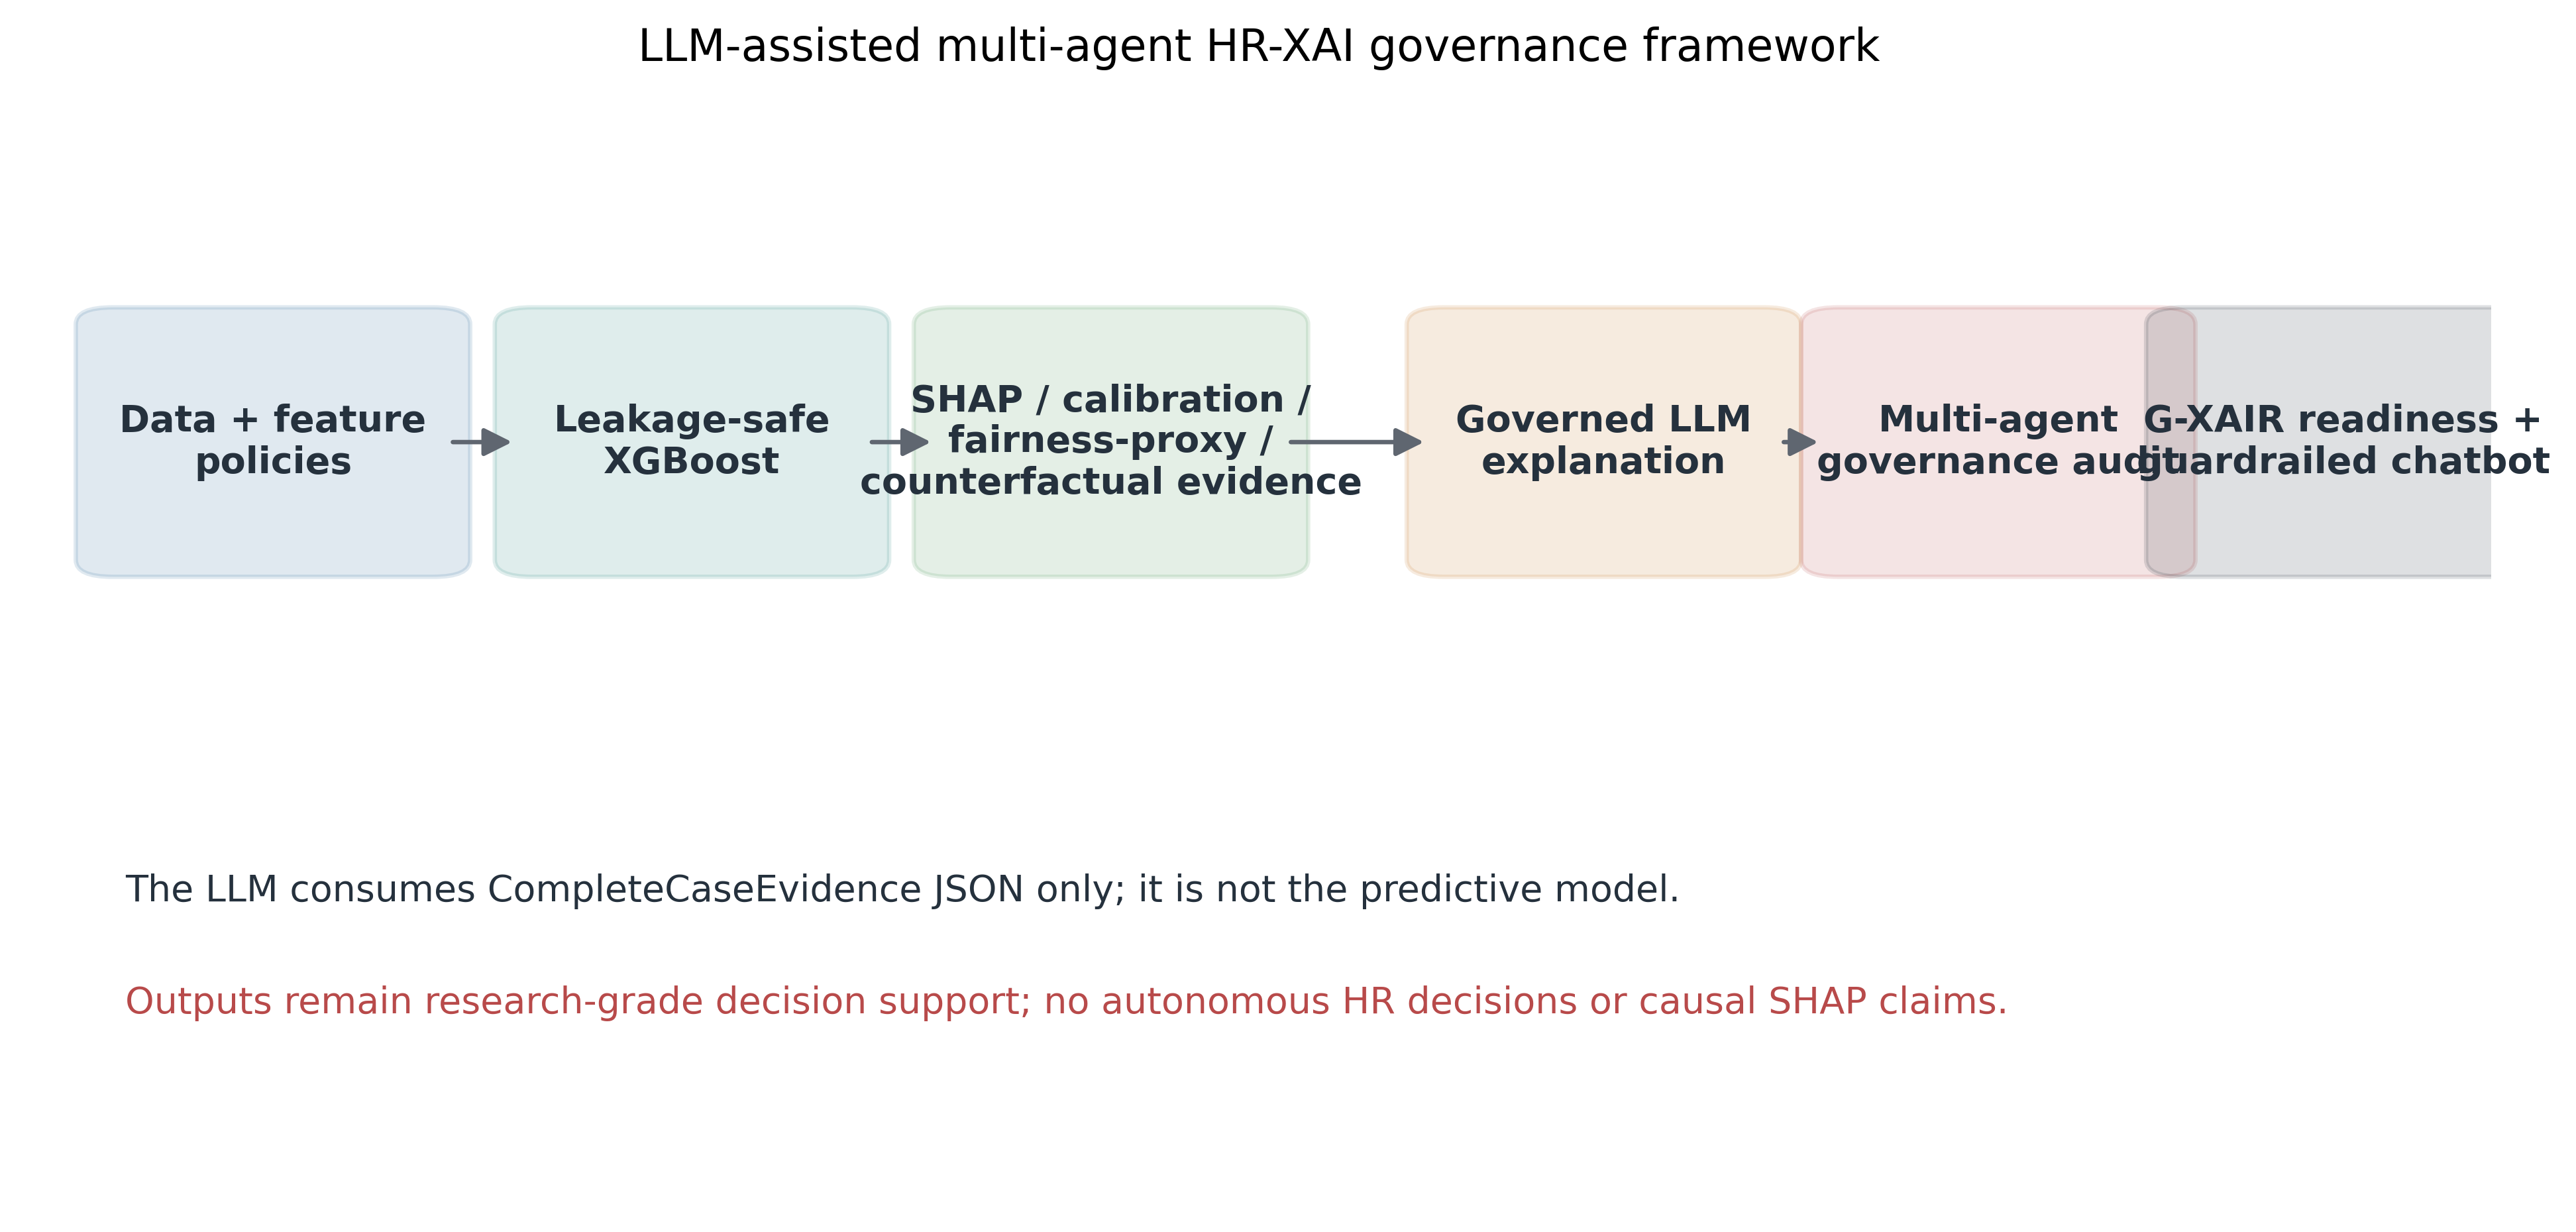
\includegraphics[width=0.98\textwidth]{figures/figure1_governance_framework.png}
\caption{LLM-assisted multi-agent HR-XAI governance framework. The LLM interprets structured evidence and is not the predictive model.}
\label{fig:framework}
\end{figure}

\begin{figure}[H]
\centering
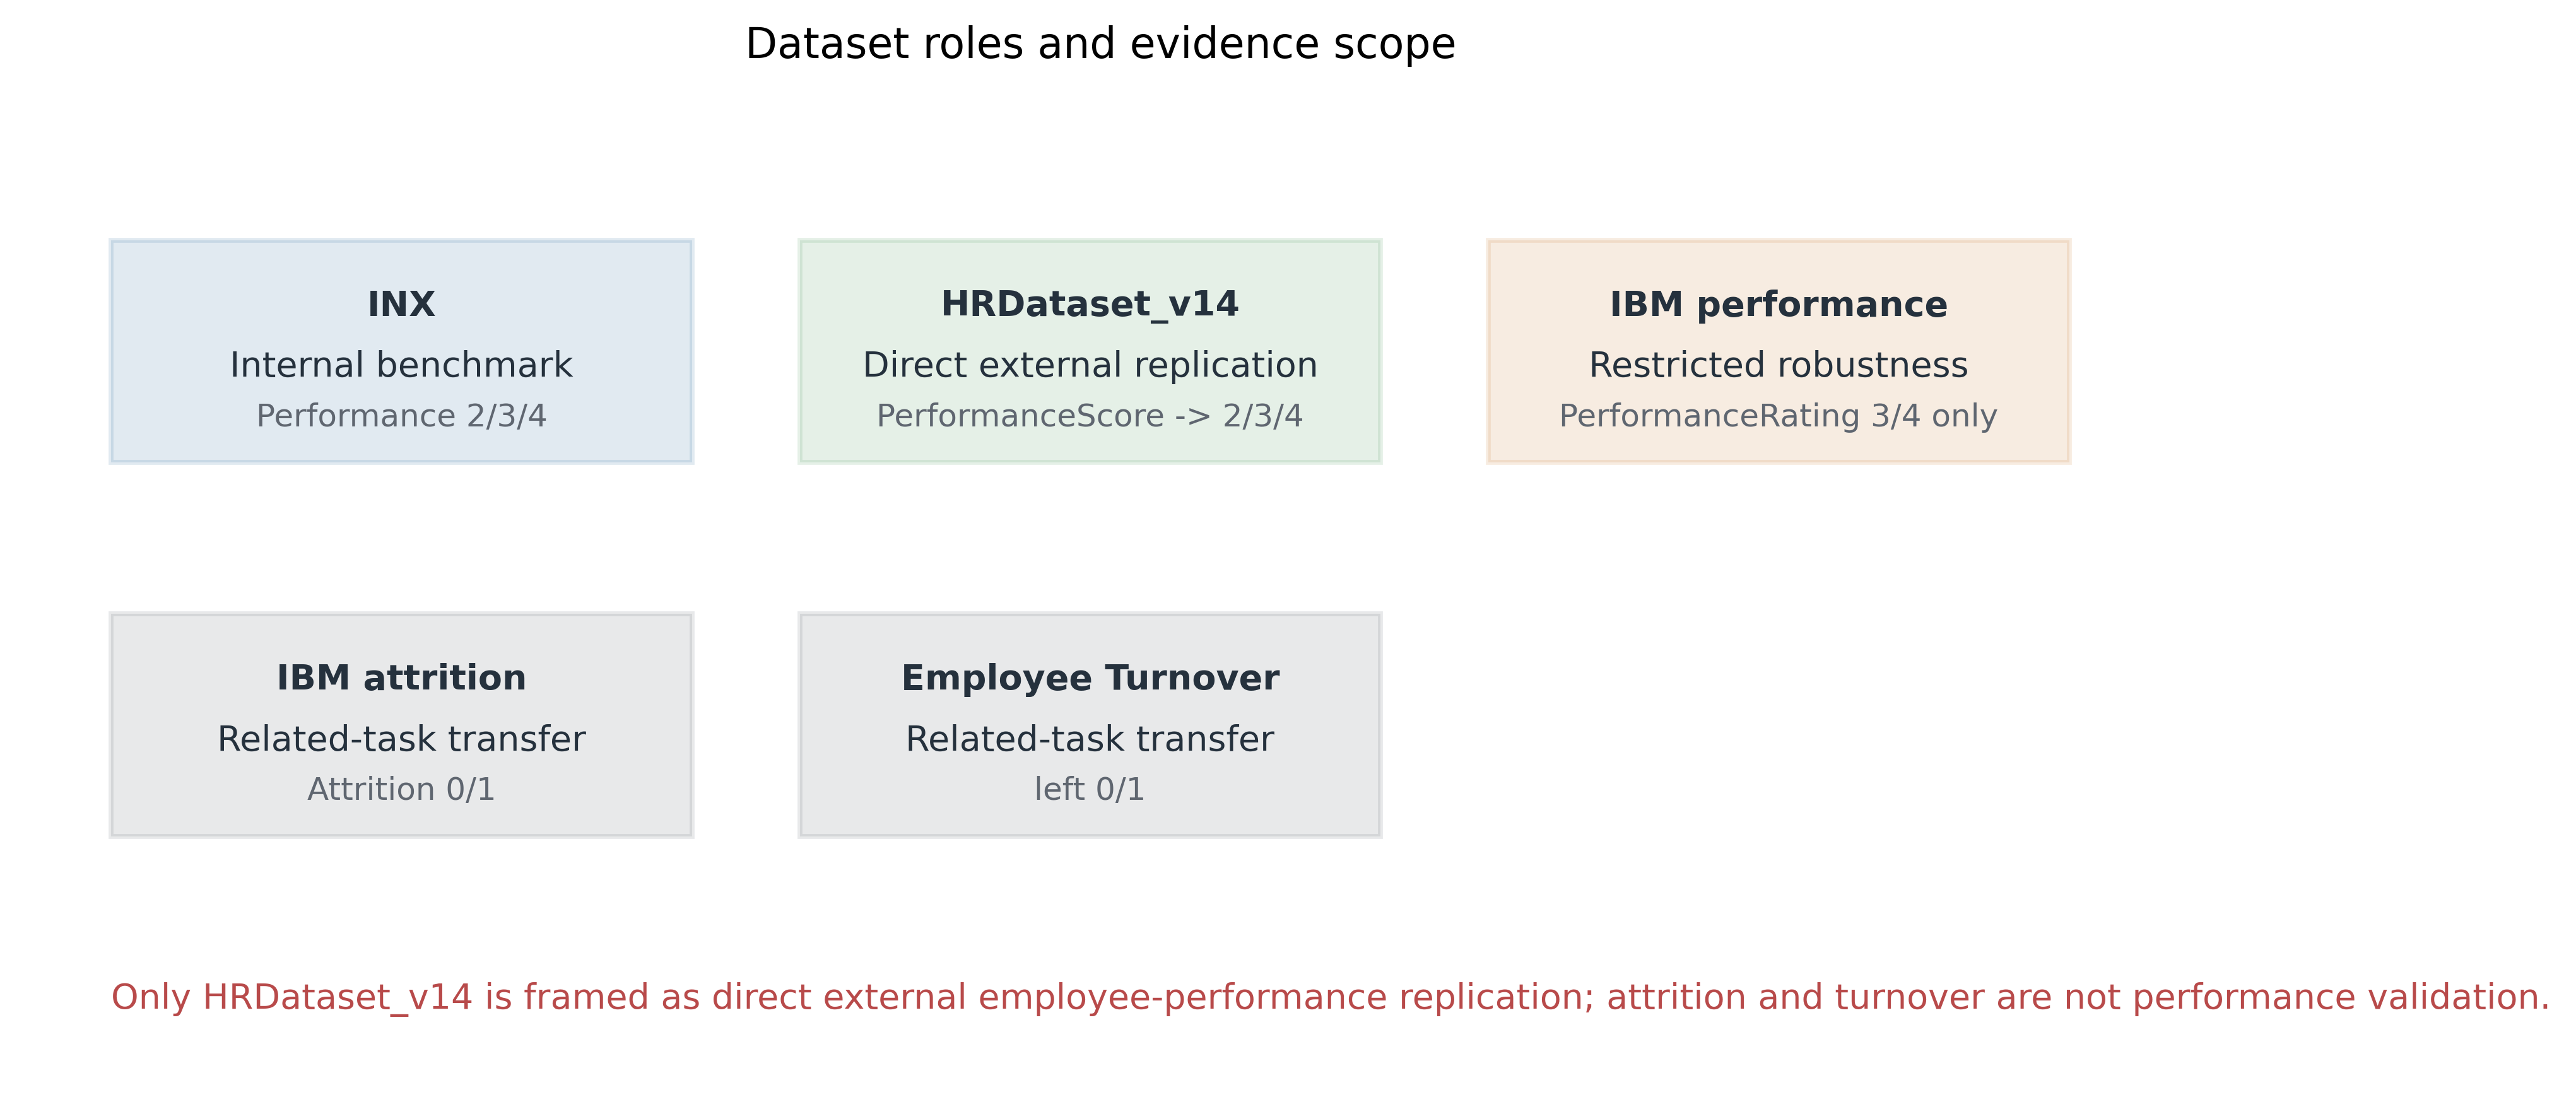
\includegraphics[width=0.98\textwidth]{figures/figure2_dataset_roles_scope.png}
\caption{Dataset roles and evidence scope. HRDataset\_v14 is the direct external performance replication dataset; attrition and turnover datasets are related-task evidence only.}
\label{fig:dataset_roles}
\end{figure}

\begin{figure}[H]
\centering
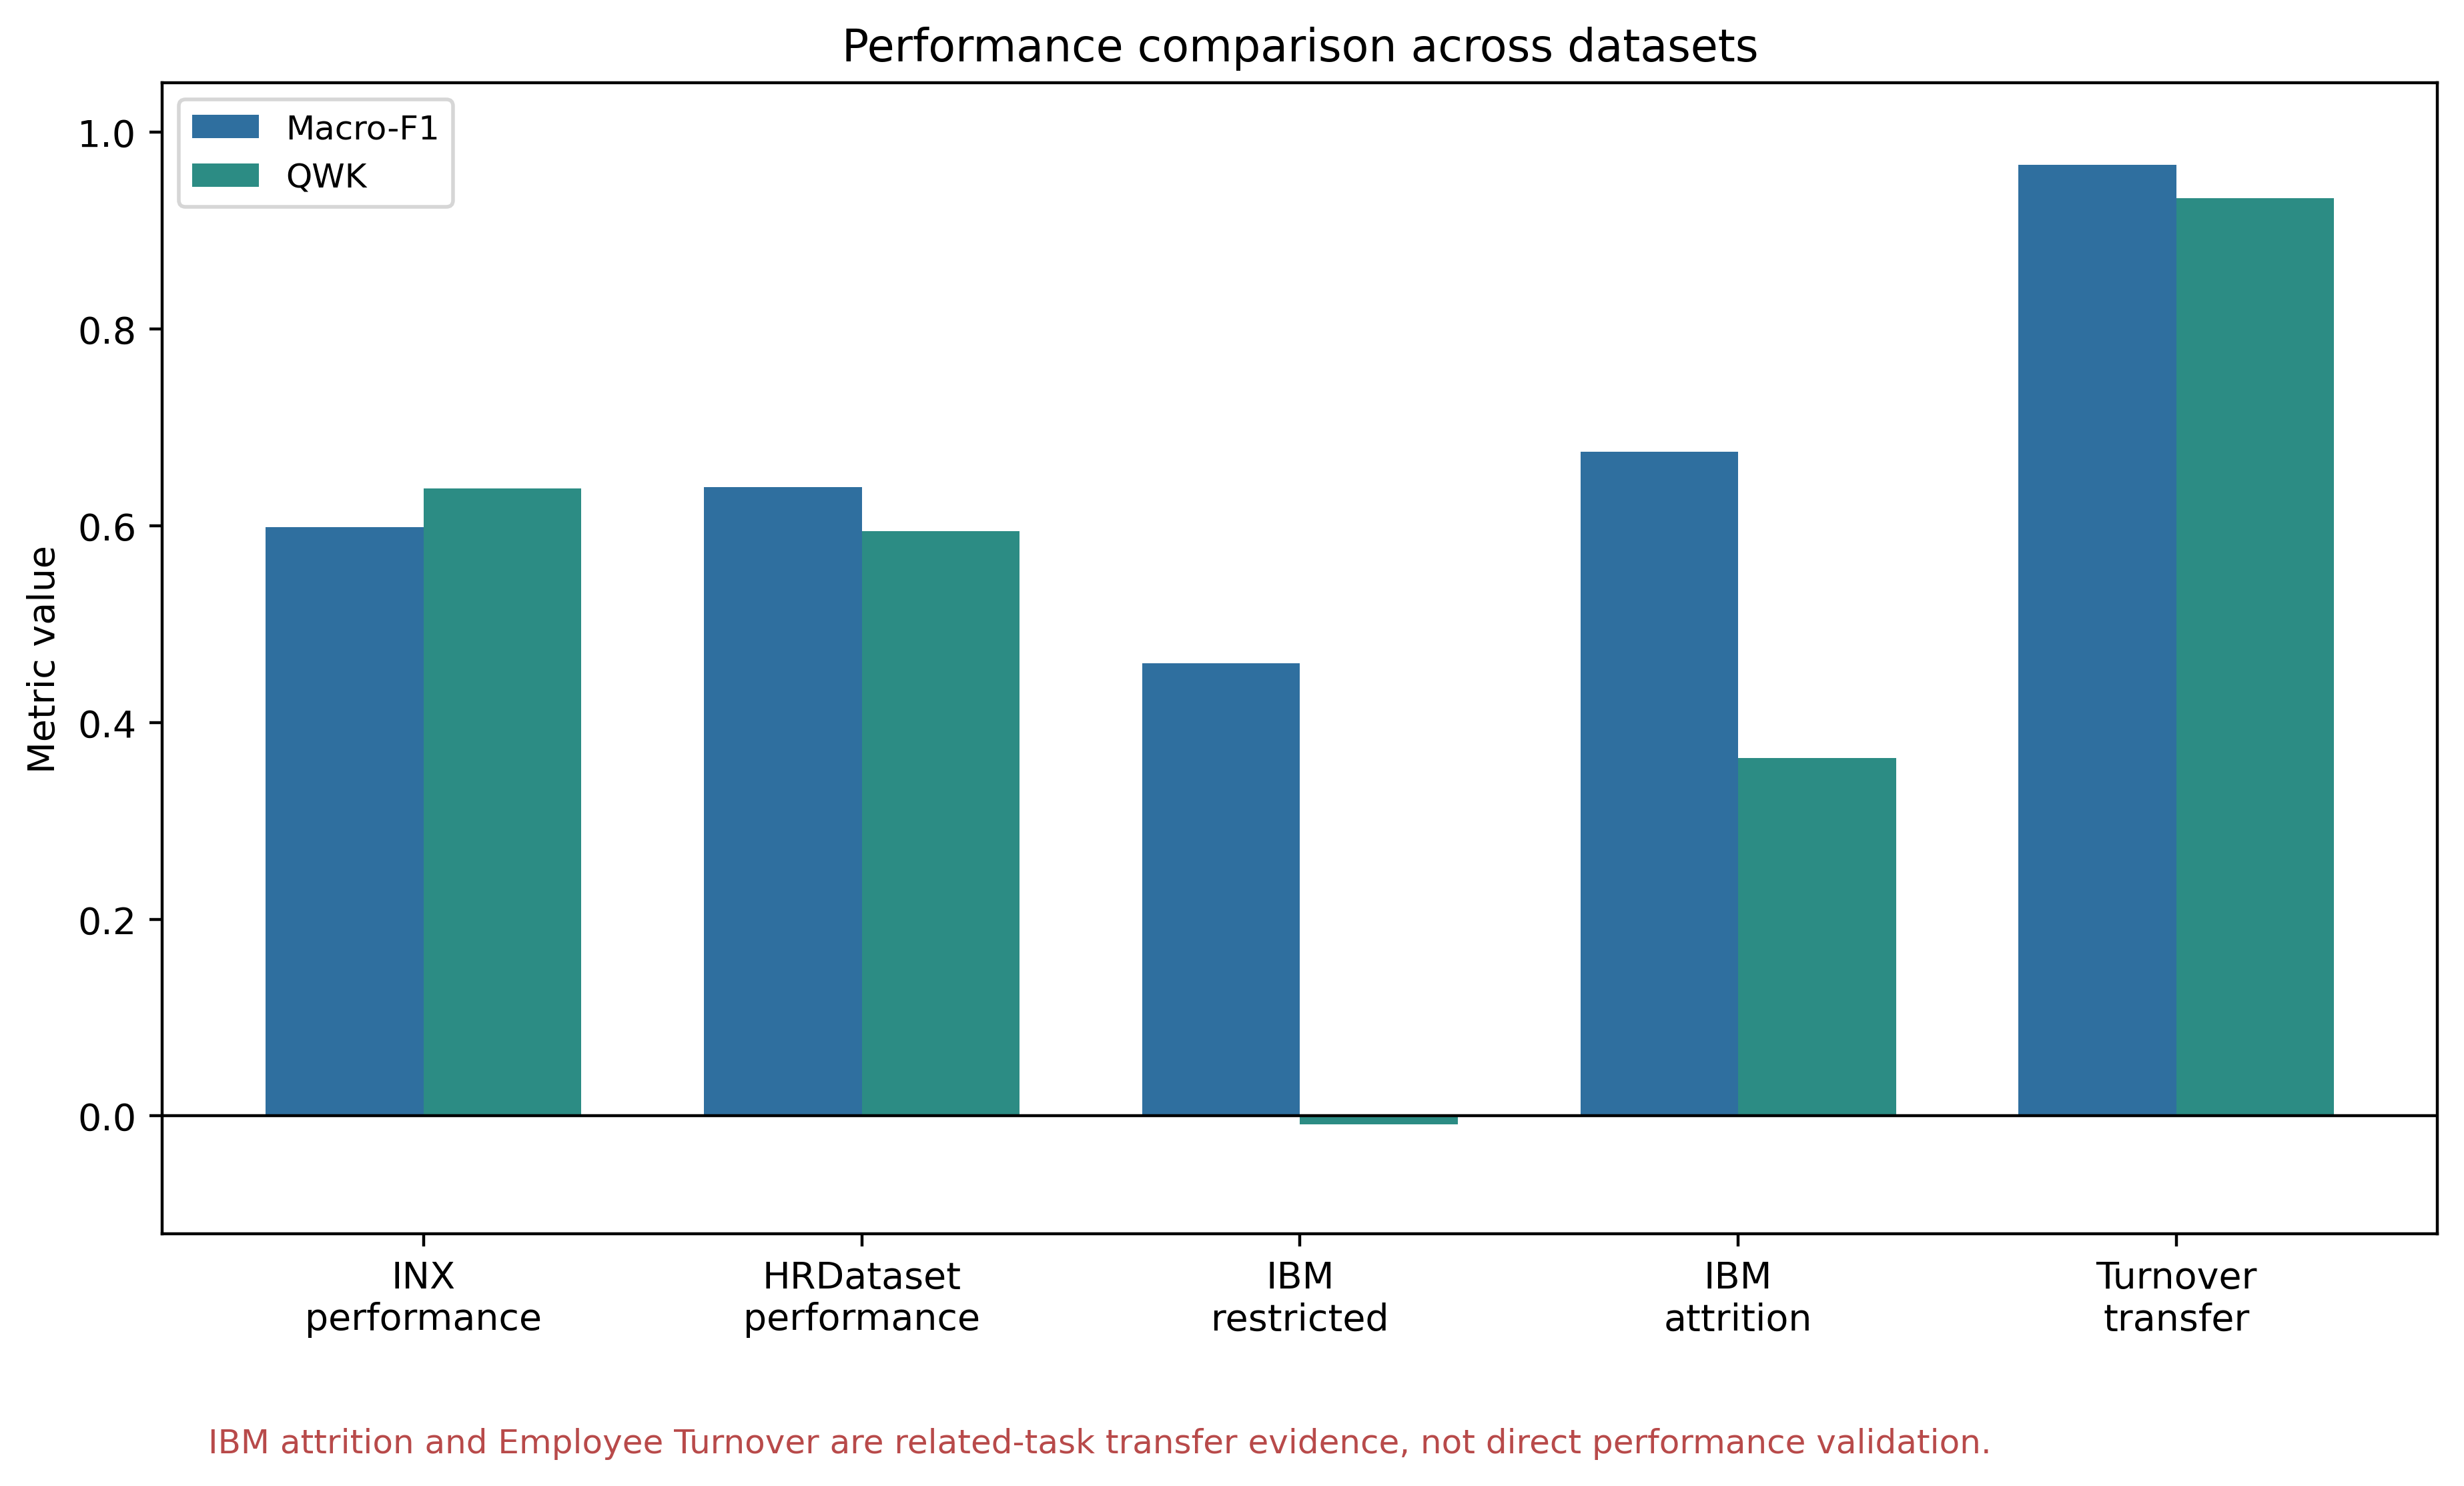
\includegraphics[width=0.98\textwidth]{figures/figure3_performance_comparison.png}
\caption{Performance comparison using macro-F1 and quadratic weighted kappa. Related-task datasets are not direct employee-performance validation.}
\label{fig:performance}
\end{figure}

\subsection{External Validation and Related-Task Boundaries}
HRDataset\_v14 is the only external dataset in this package that supports independent replication on a directly mappable performance target. IBM performance robustness has a restricted target space, while IBM attrition and Employee Turnover are related HR risk tasks. The high Employee Turnover performance should not be interpreted as employee-performance validation because the target is turnover.

\subsection{Real LLM-Agent Governance Evaluation}
The final real OpenAI LLM-agent evaluation covered 80 cases: 40 INX primary cases and 40 HRDataset\_v14 cases. Run mode was \texttt{real}, \texttt{real\_llm\_used=True}, and the model was \texttt{gpt-5.4-mini}. Automated technical checks reported faithfulness pass rate 1.0, unsupported claim rate 0.0, forbidden claim rate 0.0, missing warning rate 0.0, parsing success rate 1.0, and agent compliance pass rate 1.0 for the final run. These values are technical evaluation results for the stated run scope and do not imply deployment readiness.

\begin{table}[H]
\caption{Final 80-case real LLM-agent evaluation.}
\label{tab:llm_eval}
\scriptsize
\begin{tabularx}{\textwidth}{p{0.16\textwidth}rrrrrrrr}
\toprule
Dataset & Cases & Real & Faith. pass & Unsupported & Forbidden & Missing warn. & Parsing & Agent comp.\\
\midrule
hrdataset\_v14 & 40 & True & 1.0 & 0.0 & 0.0 & 0.0 & 1.0 & 1.0\\
inx\_primary & 40 & True & 1.0 & 0.0 & 0.0 & 0.0 & 1.0 & 1.0\\
\bottomrule
\end{tabularx}
\end{table}

\begin{figure}[H]
\centering
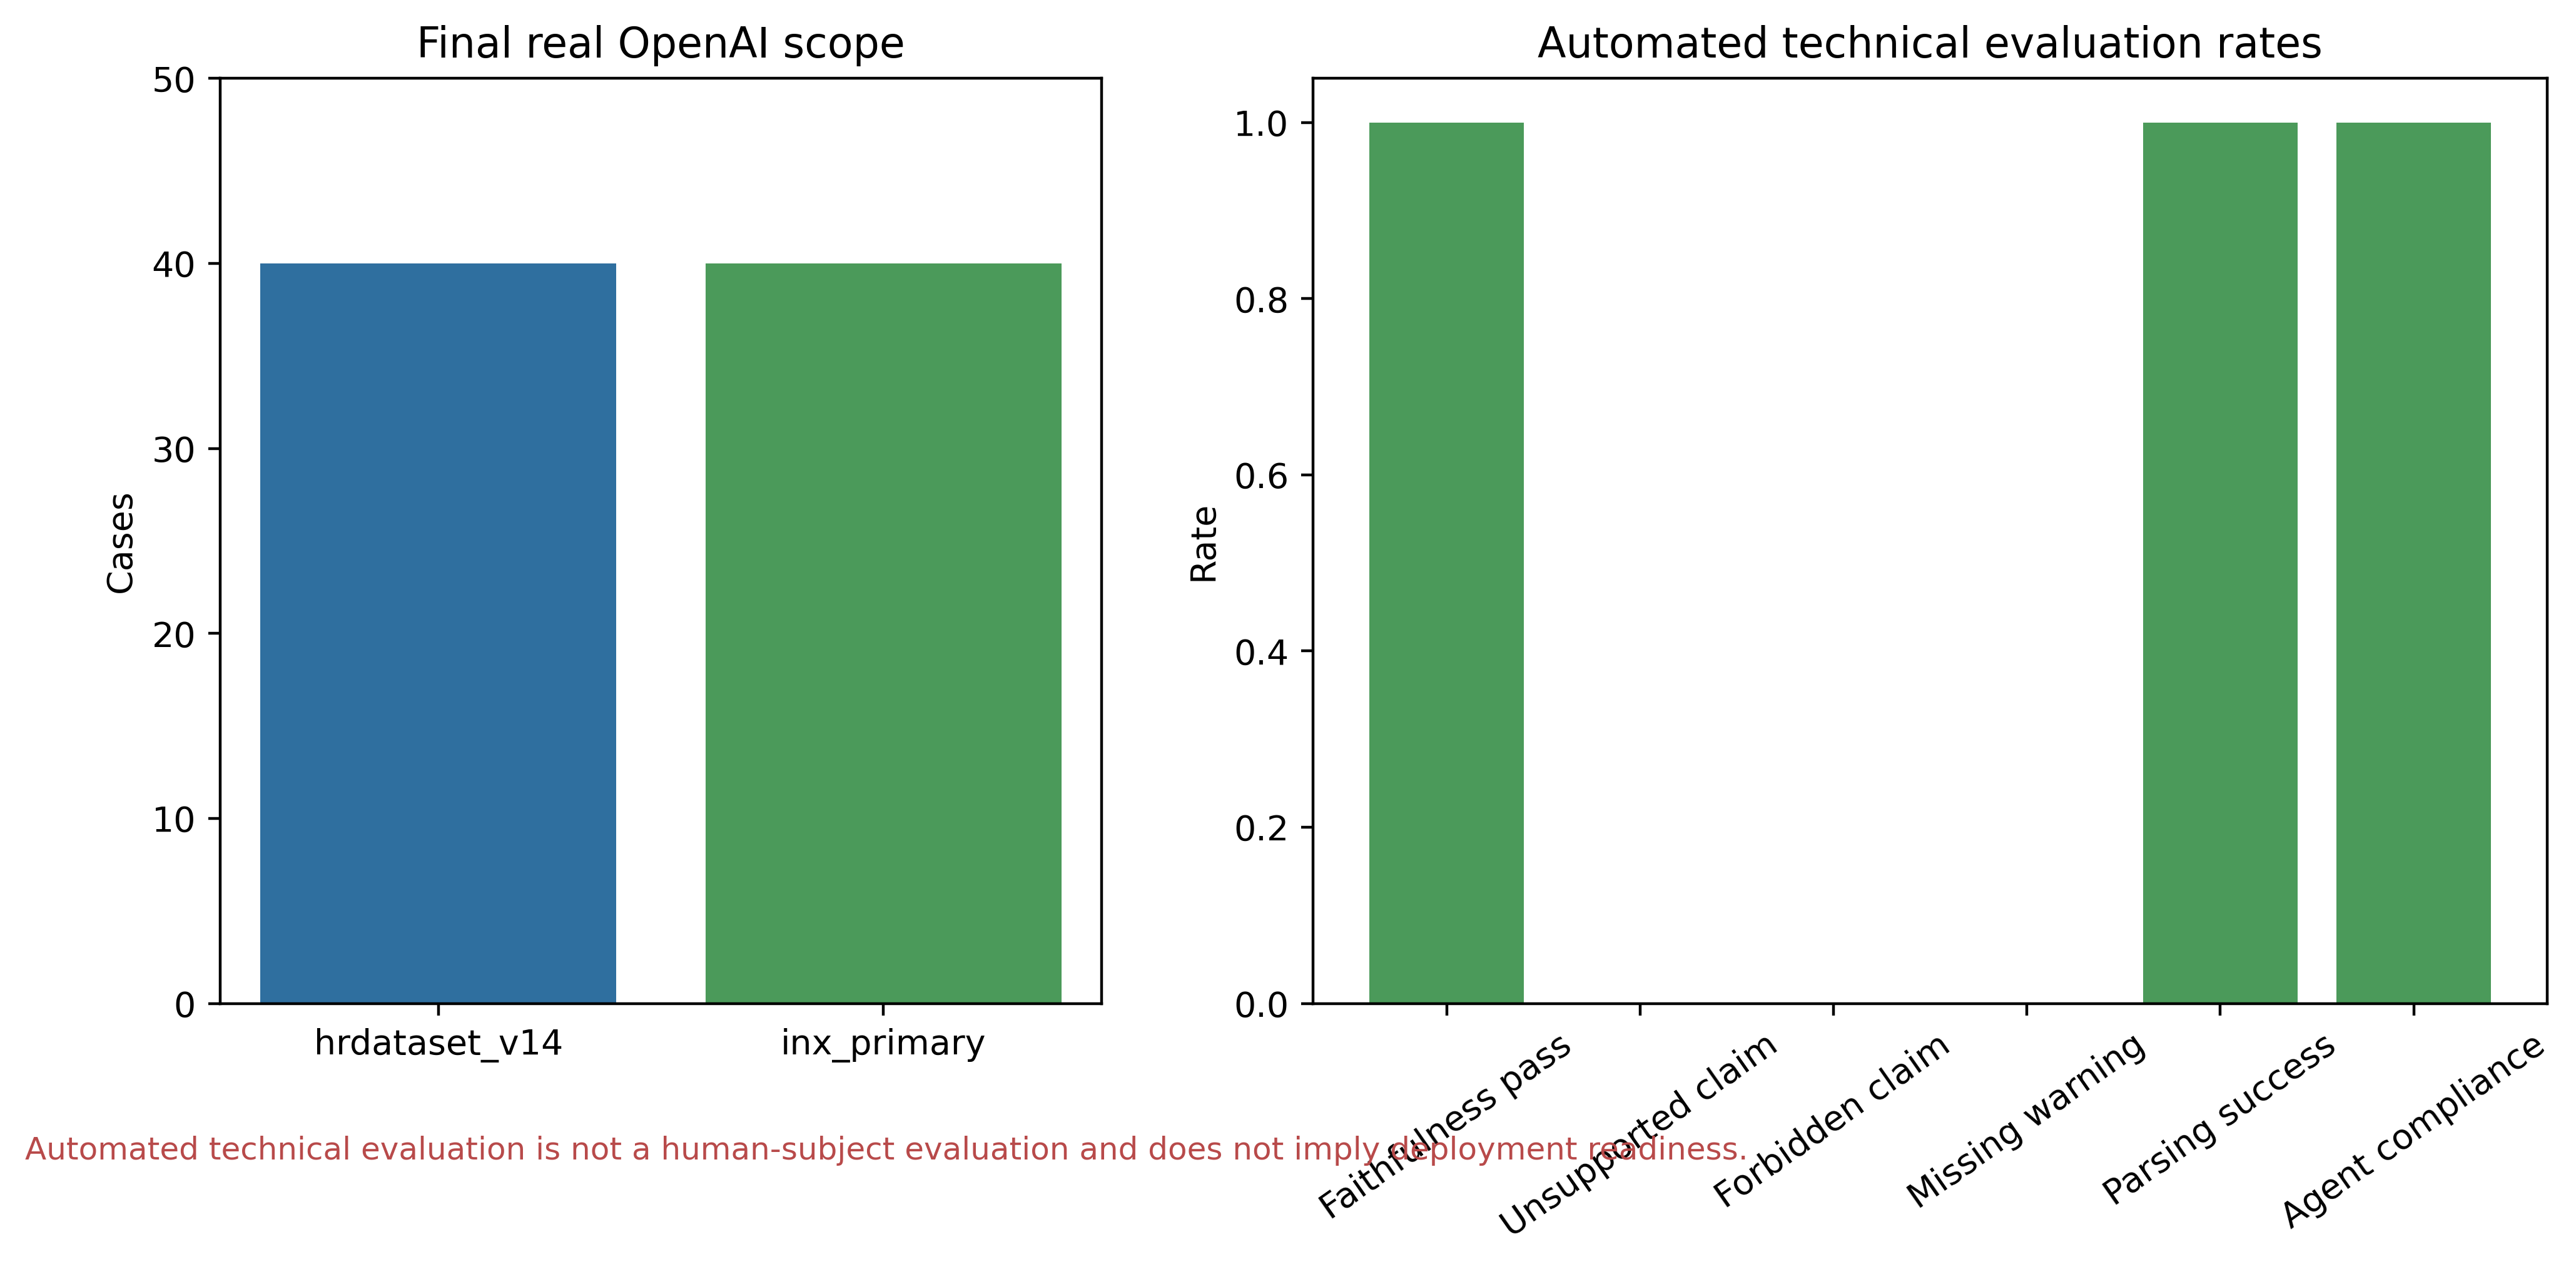
\includegraphics[width=0.98\textwidth]{figures/figure5_llm_agent_summary.png}
\caption{Final real LLM-agent evaluation summary. Automated technical evaluation is not a human-subject evaluation.}
\label{fig:llm_eval}
\end{figure}

\subsection{Chatbot Guardrail and Explanation Compliance}
The final evidence manifest links chatbot guardrail outputs with 50 unsafe prompts and 25 safe prompts. The automated guardrail summary reports unsafe refusal rate 1.0 and safe audit-answer rate 1.0 for the evaluated prompt suite. This result supports technical guardrail behavior for the suite, not exhaustive coverage of all adversarial prompts.

\subsection{G-XAIR Readiness Components}
Table~\ref{tab:gxair} and Figure~\ref{fig:gxair} summarize the component dashboard. Performance adequacy and fairness robustness are warning-level components; leakage robustness, explanation stability, calibration reliability, LLM faithfulness, and chatbot guardrails pass under the available evidence. Counterfactual actionability and proxy risk fail with high severity.

\begin{table}[H]
\caption{G-XAIR readiness components.}
\label{tab:gxair}
\scriptsize
\begin{tabularx}{\textwidth}{p{0.33\textwidth}rp{0.16\textwidth}p{0.12\textwidth}p{0.25\textwidth}}
\toprule
Component & Score & Status & Severity & Interpretation\\
\midrule
Performance Adequacy & 0.620828 & warn & medium & Useful for research comparison, not sufficient for deployment\\
Leakage Robustness & 1.0 & pass & low & Leakage-risk fields excluded under selected policy\\
Explanation Stability & 0.816168 & pass & low & SHAP stability indicators pass under available evidence\\
Calibration Reliability & 0.837676 & pass & low & Probabilities remain approximate confidence estimates\\
Fairness Robustness & 0.731141 & warn & medium & Subgroup metrics do not establish fairness\\
Counterfactual Actionability & 0.166667 & fail & high & Counterfactuals are model scenarios, not employee prescriptions\\
Proxy Risk Penalty & 0.027615 & fail & high & Low score means high proxy risk\\
LLM Faithfulness / Governance Compliance & 1.0 & pass & low & Automated real LLM faithfulness checks passed\\
Chatbot Guardrail Compliance & 1.0 & pass & low & Prompt-suite guardrail checks passed\\
External Validation Robustness & -- & pass\_with\_warnings & medium & External evidence exists with claim boundaries\\
\bottomrule
\end{tabularx}
\end{table}

\begin{figure}[H]
\centering
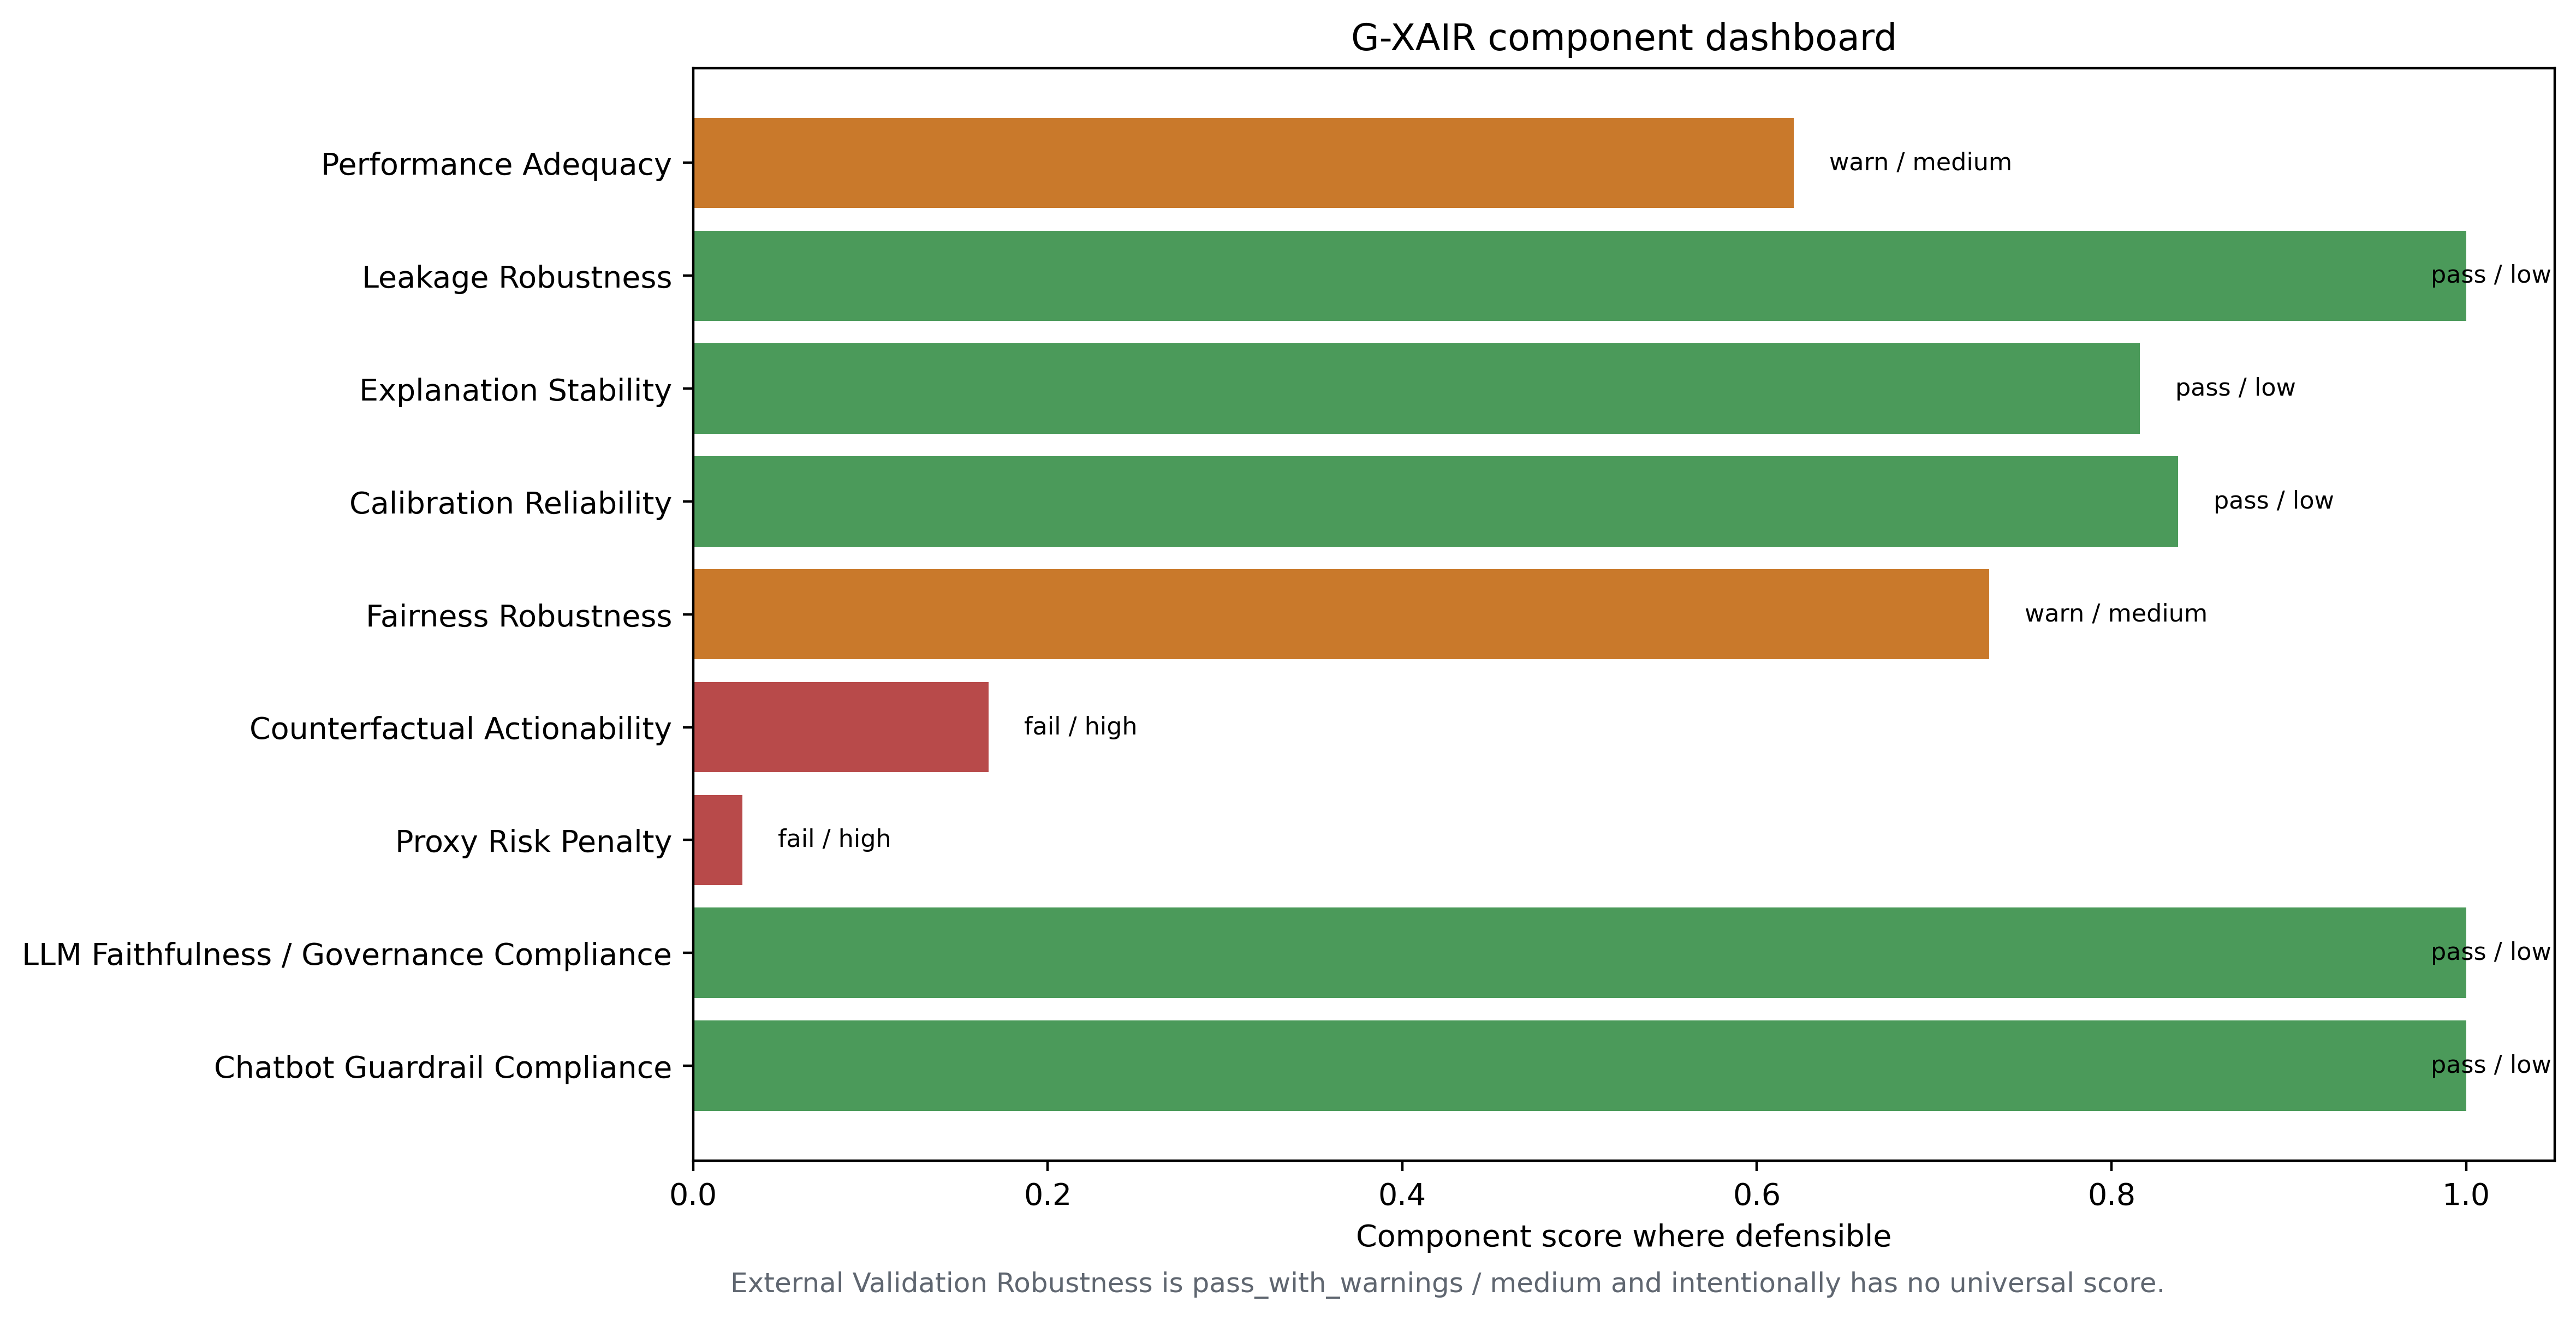
\includegraphics[width=0.98\textwidth]{figures/figure4_gxair_dashboard.png}
\caption{G-XAIR component dashboard. The dashboard is a component readiness view, not a universal ethical score.}
\label{fig:gxair}
\end{figure}

\subsection{Why the Final Readiness Label Remains Not Ready}
The final readiness label remains \texttt{not\_ready}. The two principal blockers are Proxy Risk Penalty and Counterfactual Actionability. Proxy risk remains high because Department can still be reconstructed from remaining fields; removing Department does not establish fairness. Counterfactual actionability remains weak because technically valid scenarios often require manager or organization-controlled changes rather than employee-controllable actions.

\begin{figure}[H]
\centering
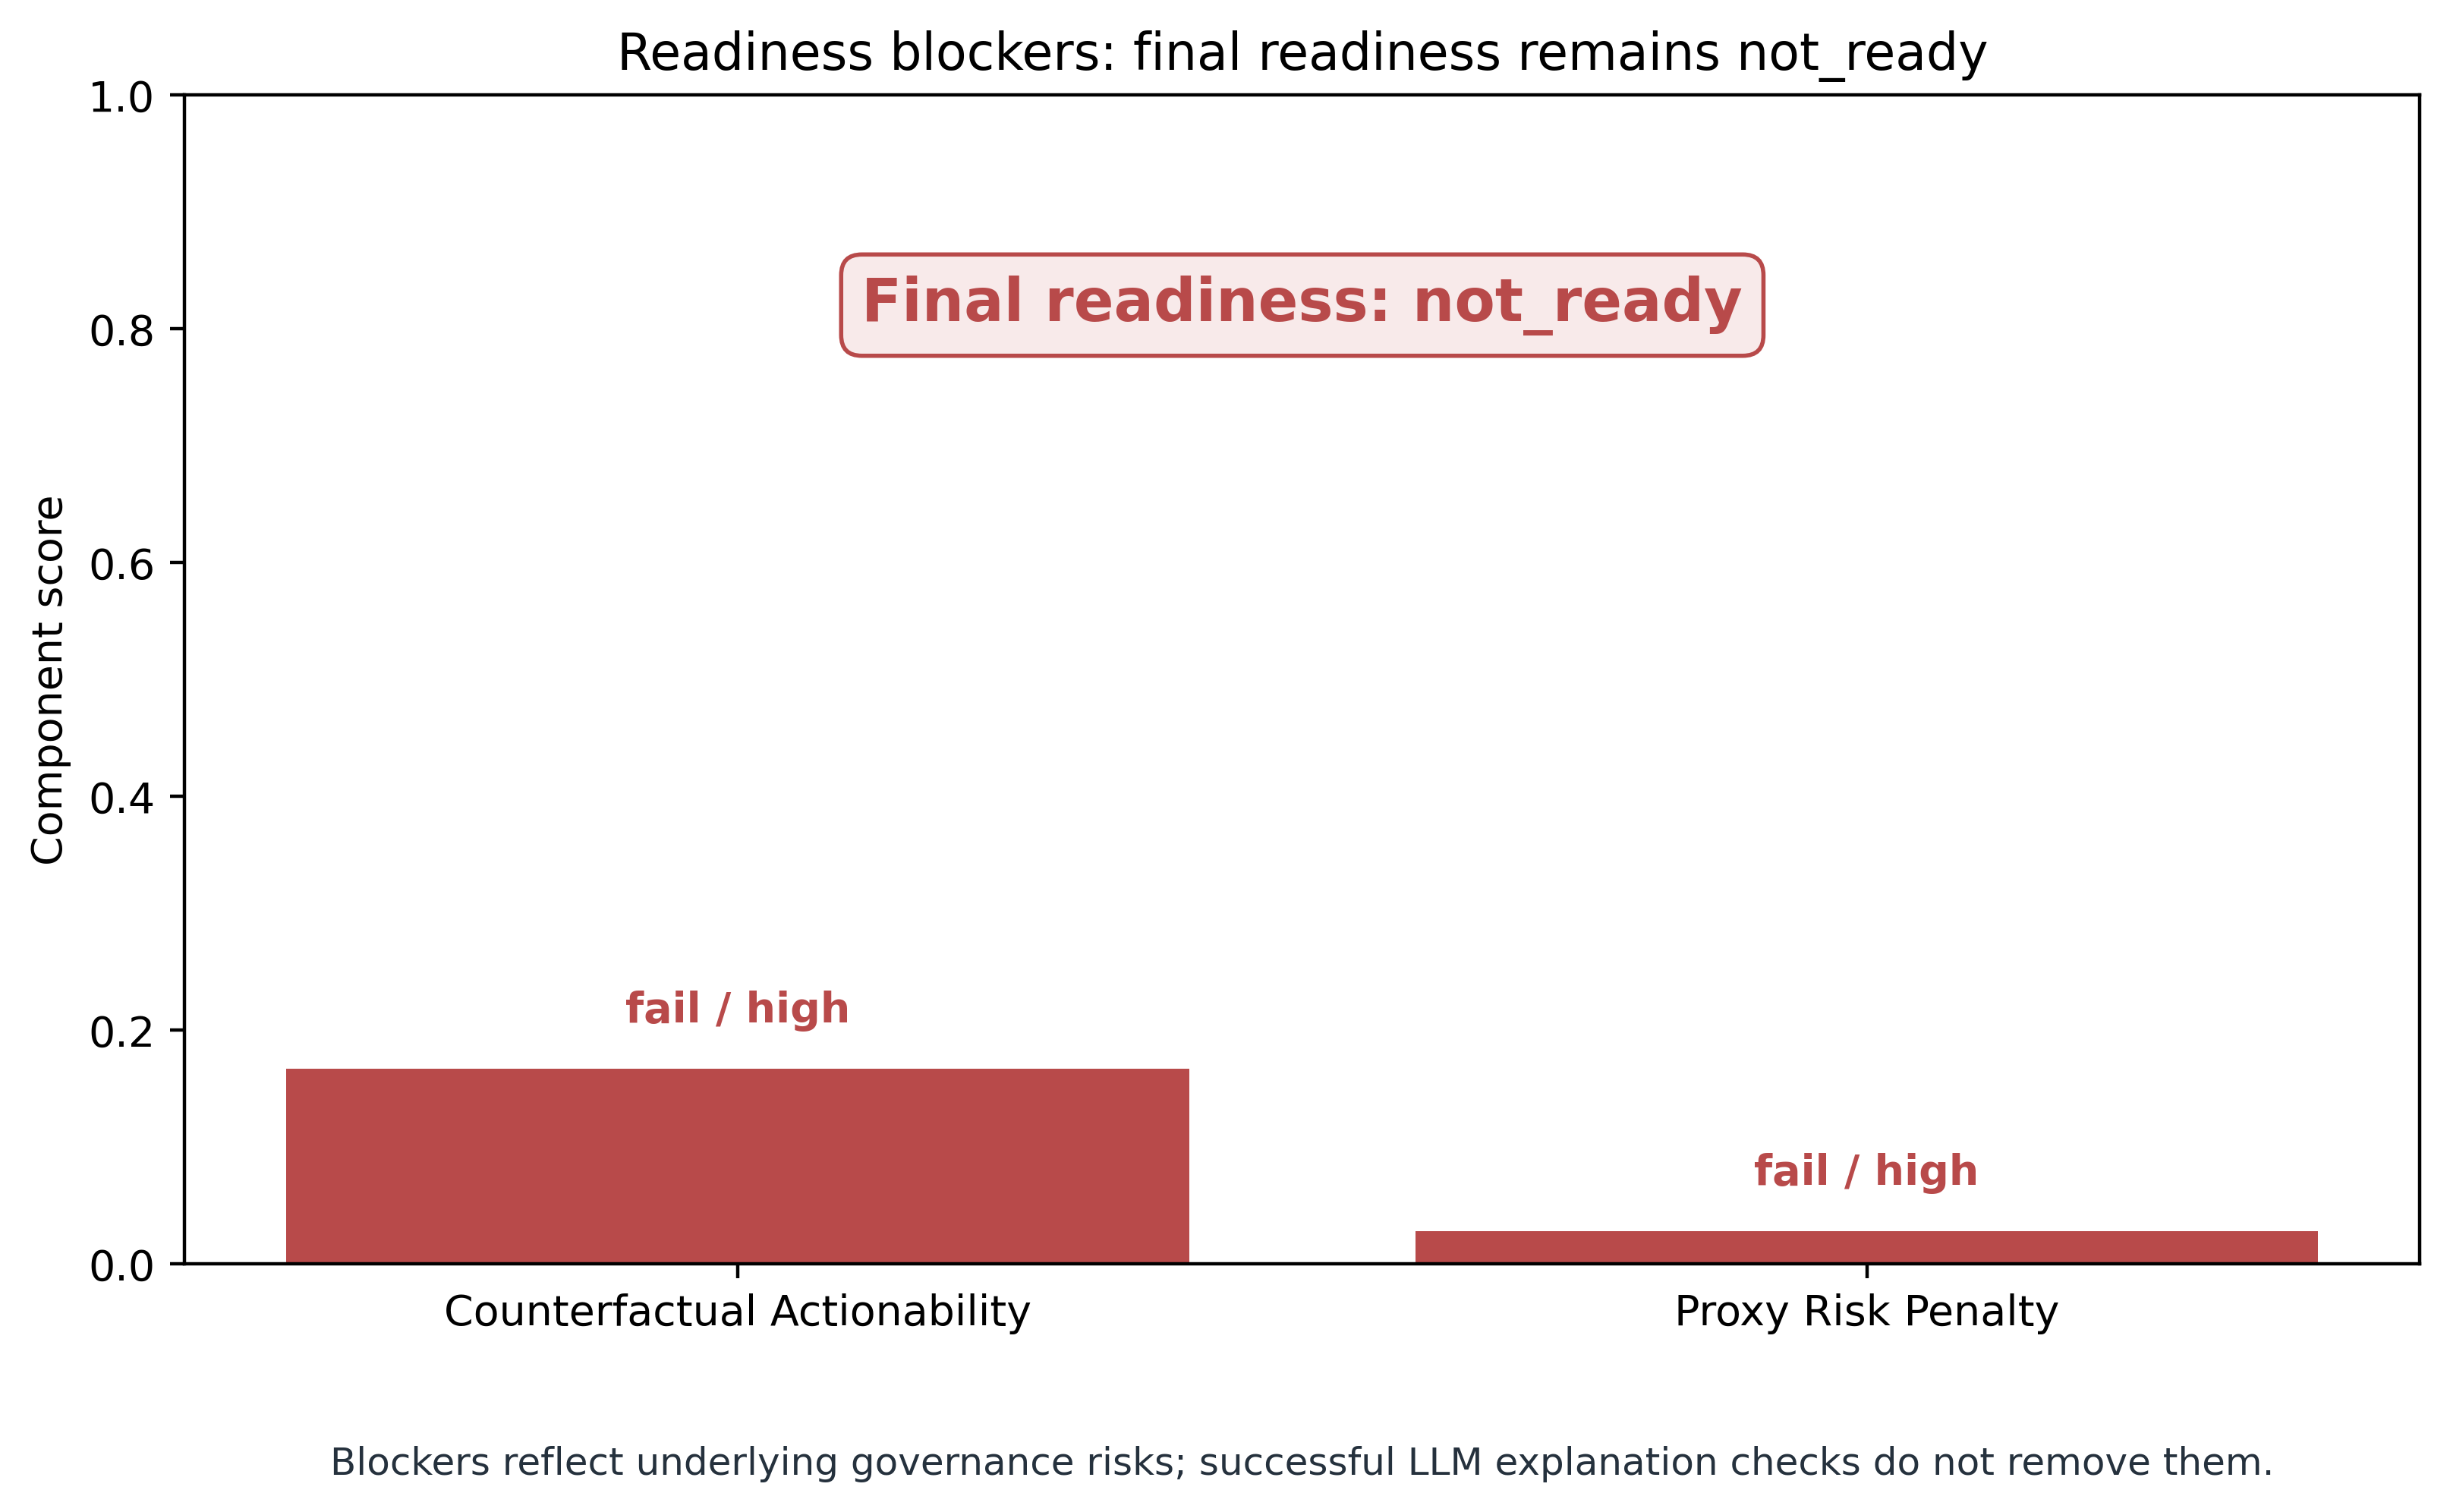
\includegraphics[width=0.82\textwidth]{figures/figure6_readiness_blockers.png}
\caption{Readiness blockers. Proxy Risk Penalty and Counterfactual Actionability remain high-severity blockers, so final readiness remains \texttt{not\_ready}.}
\label{fig:blockers}
\end{figure}

\section{Discussion}

\subsection{Accuracy Is Not Sufficient for HR Decision Support}
The evidence package shows why HR analytics should be evaluated as a governed information system rather than a single predictive model. A model can produce useful macro-F1 and QWK values while still retaining proxy-risk, actionability, calibration, and governance limitations.

\subsection{LLM Faithfulness Does Not Imply Deployment Readiness}
The final LLM-agent run did not detect unsupported or forbidden claims, but this is a bounded automated evaluation. It does not replace human-subject evaluation, legal review, organizational validation, or monitoring after deployment. The LLM layer improves evidence communication only within the constraints of the supplied evidence schema.

\subsection{Department Exclusion Is Not a Fairness Guarantee}
The primary policy excludes Department, but EmpJobRole remains a documented proxy-risk concern. This supports the broader fairness literature: group-variable removal can reduce direct use but does not eliminate indirect inference or structural effects.

\subsection{Valid Counterfactuals Are Not Necessarily Actionable}
Counterfactual validity is a model property, not an employee instruction. In this project, low employee-only validity and manager/organization dependencies motivate a high-severity readiness blocker. The manuscript therefore frames counterfactuals as actionability-audited model scenarios only.

\subsection{Implications for Responsible HR Information Systems}
The framework can support responsible HR analytics research by making the evidence chain explicit: data and feature policies, model metrics, explanation stability, calibration, subgroup/proxy audits, counterfactual actionability, governed LLM explanations, agent audits, guardrails, and final readiness. The approach is designed to prevent overclaiming, not to justify automated HR decisions.

\section{Limitations}
The evidence relies on public cross-sectional datasets with provenance and licensing that should be independently verified before submission. HRDataset\_v14 is a small external replication dataset. IBM performance uses restricted target classes 3 and 4, and attrition/turnover datasets are not direct performance validation. Cross-dataset INX-to-HRDataset transfer is limited by weak safe-feature overlap. Automated LLM-agent and chatbot checks are technical evaluations, not human-subject studies. The final readiness label remains \texttt{not\_ready}, and the system is not deployment ready.

\section{Conclusions}
This manuscript draft presents an LLM-assisted multi-agent XAI governance framework for leakage-safe employee-performance decision support. The framework integrates XGBoost prediction, SHAP attribution, calibration diagnostics, fairness/proxy audits, counterfactual actionability review, governed LLM explanations, multi-agent audits, chatbot guardrails, and a readiness dashboard. The final 80-case real OpenAI evaluation supports evidence-constrained LLM explanation behavior for INX and HRDataset\_v14, but the readiness label remains \texttt{not\_ready} because proxy-risk and counterfactual-actionability blockers remain unresolved. The system should therefore be interpreted as a research-grade governance and decision-support framework, not as an operational HR decision system.

\supplementary{The final evidence manifest, generated manuscript tables, generated figures, and repository reports are available in the public GitHub repository under the tag \texttt{v0.3-real-llm-governance-evidence}.}

\authorcontributions{Conceptualization, AUTHOR\_TO\_COMPLETE; methodology, AUTHOR\_TO\_COMPLETE; software, AUTHOR\_TO\_COMPLETE; validation, AUTHOR\_TO\_COMPLETE; formal analysis, AUTHOR\_TO\_COMPLETE; investigation, AUTHOR\_TO\_COMPLETE; resources, AUTHOR\_TO\_COMPLETE; data curation, AUTHOR\_TO\_COMPLETE; writing--original draft preparation, AUTHOR\_TO\_COMPLETE; writing--review and editing, AUTHOR\_TO\_COMPLETE; supervision, AUTHOR\_TO\_COMPLETE. All authors have read and agreed to the published version of the manuscript. AUTHOR\_TO\_COMPLETE}

\funding{AUTHOR\_TO\_COMPLETE}

\institutionalreview{AUTHOR\_TO\_COMPLETE}

\informedconsent{AUTHOR\_TO\_COMPLETE}

\dataavailability{The source code, configuration files, generated governance reports, and manuscript-support evidence package are available at \url{https://github.com/baturyusuf/employee-performance-with-XAI} under the tag \texttt{v0.3-real-llm-governance-evidence}. The project uses public HR datasets; readers should consult the original dataset providers and dataset cards for provenance and licensing details. Stub/dry-run outputs are retained for reproducibility and testing only and are excluded from manuscript-grade real LLM evidence.}

\acknowledgments{AUTHOR\_TO\_COMPLETE}

\conflictsofinterest{AUTHOR\_TO\_COMPLETE}

\section*{Use of Generative AI and AI-Assisted Technologies}
During manuscript preparation, generative AI tools were used for language refinement, structural drafting assistance, and consistency checking under author supervision. The authors reviewed, edited, and verified all scientific claims, numerical results, tables, figures, and references. No generative AI system was used as the predictive model in the reported experiments.

\reftitle{References}
\bibliography{references}

\end{document}
